%Sample for icsthesis.cls
%Author: JCEPlaras
%Reminders: Omit \lipsum commands

\documentclass{icsthesis}
\usepackage{lipsum} %for generating dummy text

%\usepackage{showframe} %for debugging the margins
                              
                              
%Replace the values here, various commands depend on this variables                                                                                                                                                            
\renewcommand{\TITLE}{AN ATTEMPT TO SOLVE THE P=NP PROBLEM USING MATCHES STONES AND STICKS TO REPRESENT M-TAPE N-HEAD TURING MACHINES}
\renewcommand{\AUTHOR}{JEJOMAR B. ARROYO}
\renewcommand{\DEGREE}{MASTER OF SCIENCE}
\renewcommand{\MAJOR}{COMPUTER SCIENCE}
\renewcommand{\MONTH}{JANUARY}
\renewcommand{\YEAR}{2060}

\begin{document}
	
	\begin{frontmatter}
		%create title
		\maketitle
				
		\begin{approvalpage}
			The thesis hereto attached entitled \TITLE , prepared and submitted by \AUTHOR , in partial fulfillment of the requirements for the degree of \DEGREE\ (\MAJOR) is hereby accepted.
			
			\begin{multicols}{2}
				\centering
				\addsignature{ISAAC X. NEWTON}{Member, Guidance Committee} %custom command for adding signature field
				\columnbreak
				\addsignature{ISAAC X. NEWTON}{Member, Guidance Committee}
			\end{multicols}
			\addsignature{ALAN X. TURING}{Chair, Guidance Committee}
			
			Accepted as partial fulfillment of the requirements for the degree of \DEGREE\ (\MAJOR). 
			\addsignature{EDSGER W. DIJKSTRA}{Director, Institute of Graphs}
			\addsignature{STEPHEN W. HAWKING}{Dean, Graduate School\\University of the Mars Los Ba\~{n}os}
		\end{approvalpage}
		
		\begin{biosketch}
			\lipsum[4] %insert dummy text
			
			MUST NOT EXCEED ONE PAGE.		
			
			\addauthorsignaturefield
		\end{biosketch}	
		
		%acknowledgement
		\begin{acknowledgement}
			\lipsum[4]
			\lipsum[4]
			\lipsum[4]
			MUST NOT EXCEED ONE PAGE.
		\end{acknowledgement}
		
		%TOC
		\maketableofcontents
		
		%LOT
		\makelistoftables

		%LOF
		\makelistoffigures
	
		%ABSTRACT
		\begin{abstractwithpageno}
			\lipsum[4]MUST NOT EXCEED ONE PAGE.
		\end{abstractwithpageno}

	\end{frontmatter}
	
	%BODY OF THESIS HERE (Use up to 3 levels only, (sec -> subsec -> subsubsec)
	\begin{mainmatter}
		\section{INTRODUCTION}
			\subsection{Major Subsection}
				\lipsum[4]
			\subsection{Major Subsection}
				\lipsum
		
		\section{REVIEW OF LITERATURE}
			\subsection{Here Subsection}
				\lipsum[4]
				\subsubsection{Apa Subsubsection}
					APA CITATION SAMPLE HERE USING BIBTEX \citep{CrescenziKann1997}
				\subsubsection{Wooo subsubsection}
					\lipsum
			\subsection{Here Subsection}
				\lipsum[6]
				
				
		
		\section{METHODOLOGY}
			\lipsum[1]
			
			%FIGURE INSERTION SAMPLE
			\begin{figure}[ht]
			\begin{center}
				\vspace{4ex}
				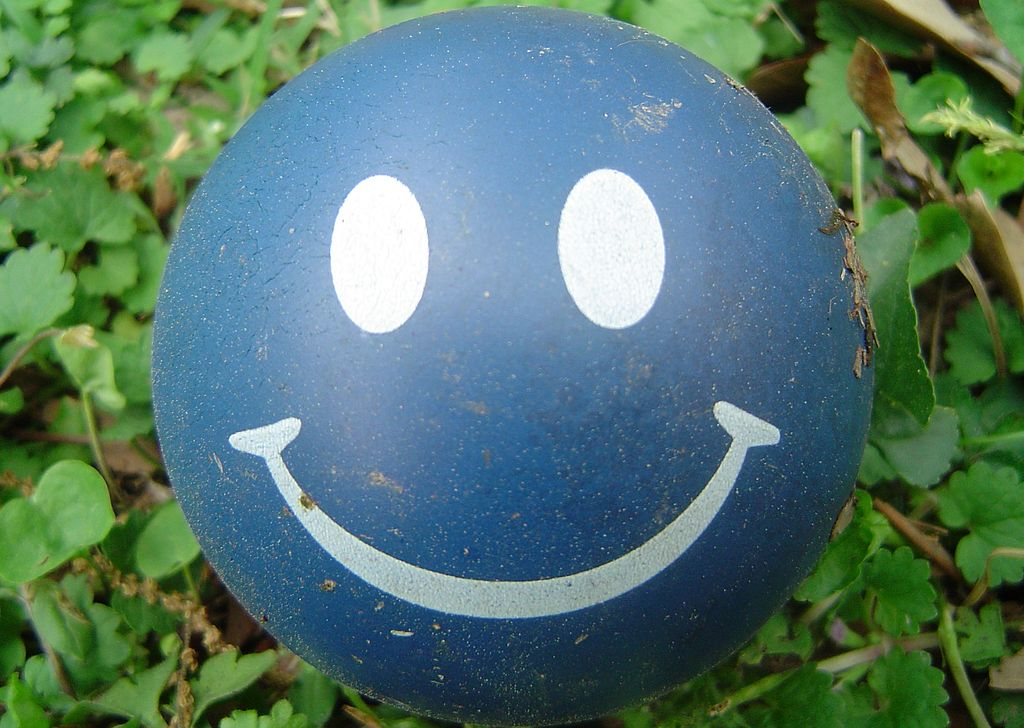
\includegraphics[width=200px]{figuretest}
				\label{fig:Test Caption Figure}	
				\caption{Test Caption Figure}
			\end{center}
			\end{figure}
			
			\lipsum
		
		\section{RESULTS AND DISCUSSION}
			\lipsum[4]
			
			%TABLE INSERTION SAMPLE
			\begin{table}[ht]
			\vspace{4ex}
			\centering
				\caption{Test Caption Table}
				
				\label{table:Test Caption Table}
				\begin{tabular}{llllll}
				\hline
				\hline
				1 & 2 & 3 & 4 & 5 & 6 \\ \hline
				1 & 2 & 3 & 4 & 5 & 6 \\
				1 & 2 & 3 & 4 & 5 & 6 \\
				1 & 2 & 3 & 4 & 5 & 6 \\ \hline\hline
				\end{tabular} 
			\vspace{4ex}
			\end{table}
			
			\lipsum[4-10]
			\lipsum[5]
		
		\section{SUMMARY AND CONCLUSION}
			\lipsum[4]
		
		%References command
		%Parameter is the references bib file without extension
		\makereferences{references}
			
	\end{mainmatter}
\end{document}
